\documentclass[10pt,twocolumn]{ctexart}
\usepackage[margin=0.65in]{geometry}
\setlength{\columnsep}{0.25in}
\usepackage{graphicx}
\usepackage{booktabs}
\usepackage{amsmath}
\usepackage{xcolor}
\usepackage{listings}
\usepackage{caption}
\captionsetup{font=small,labelfont=bf}
\lstset{basicstyle=\ttfamily\footnotesize,breaklines=true,frame=single}
\setCJKmainfont{SimSun}[AutoFakeBold=2.5]
\setCJKsansfont{Microsoft YaHei}[AutoFakeBold=2.5]
\setCJKmonofont{Microsoft YaHei}

\begin{document}

\begin{center}
{\LARGE\bfseries 基于执行反馈的 LLM 辅助移动机器人任务规划}\\[0.5em]
Jian Fangyuan/菅方源
\end{center}

\section*{Abstract}
本报告实现了一个运行于 Webots R2025a 与 ROS~2 Humble 的移动机器人任务规划系统。
系统将自然语言请求转换为少量、经过验证的高层技能调用，并遵循 Plan--Validate--Execute--Observe--Recover 闭环。
实验中 LLM 只能在固定白名单中选择技能；验证器在执行前检查每个调用；执行后系统读取结构化结果，
并在超时、障碍、窄缝等失败场景下进行有界恢复，必要时把任务级执行反馈发回 LLM 重规划。
正常任务与可重试任务 5/5 成功，2 个非法计划全部在执行前被拒绝，2 个不可恢复失败（超时、持续障碍）均及时安全停止；
成功任务平均耗时 8.65\,s，可测得的最终位置误差平均约 0.081\,m。


\section{系统架构与技能接口}
\label{sec:arch}

\subsection{整体架构}
系统由四层组成：Planner、Validator、Skill Executor、ROS~2 技能层，
执行结果再进入 Recovery，形成 Plan--Validate--Execute--Observe--Recover 闭环：


\begin{itemize}
  \item \textbf{Planner}：模拟规划器或兼容的 LLM 规划器，输出原始 \texttt{SkillCall[]}；
  \item \textbf{Validator}：六层检查，不通过则计划不会到达机器人；
  \item \textbf{Skill Executor}：只把白名单技能名映射到预定义 Python 方法；
  \item \textbf{RobotSkills}：ROS~2 节点，发布 \texttt{/agent0/cmd\_vel}，读取 GPS、罗盘与 \texttt{/scan}；
  \item \textbf{Recovery}：根据 \texttt{SkillResult} 选择 retry / backup / replan / stop。
\end{itemize}

这种分层的意义在于：LLM 可以出错，但只要它无法绕过 Validator，
最坏情况也只是计划被拒绝，而不是机器人收到危险指令。
我们没有把安全寄希望于提示词，而是把安全放在 LLM 与执行器之间。

\subsection{技能接口}
三个技能的契约如下。注册表是单一事实来源：
同一份定义既生成验证器使用的 JSON Schema，也生成 LLM 工具列表，
避免接口定义与实际执行漂移。

\begin{center}
\captionof{table}{技能接口摘要。}
\setlength{\tabcolsep}{3pt}
\footnotesize
\begin{tabular}{p{0.29\linewidth}p{0.61\linewidth}}
\toprule
技能 & 契约 \\
\midrule
\texttt{navigate\_to} &
参数 $x,y,\theta$；位置误差 $\le 0.10$ m，航向 $\le 0.15$ rad；超时 30 s \\
\texttt{follow\_waypoints} &
参数：航点列表；失败时返回最后到达的航点下标；每个航点超时 30\,s \\
\texttt{stop} &
发布零速度；成功：已发布零速度；超时：2\,s \\
\bottomrule
\end{tabular}
\end{center}

设计技能接口时，我们刻意去构造了结构化的返回值，使每个操作都可以得到一定反馈。
每个技能都返回 \texttt{success}、\texttt{reason} 和 \texttt{elapsed\_time\_s}，
因为上层恢复策略需要知道失败原因，而不仅是失败事实。
这一决定是后续执行反馈与有界重规划能够成立的前提。

\subsection{具名地点与工作空间}
当前具名地点：entrance $(0.0,3.0)$、storage $(-2.152,-1.363)$、
workbench $(4.8,0.0)$、charging\_station $(-2.17,1.95)$（可以见下面的地图）。
工作空间为 $x \in [-7,7]$、$y \in [-4,7]$。
以上坐标与 \texttt{agent/locations.py} 中的常量表一致；提示词、验证器工作空间和具名地点均由同一份定义生成，避免接口漂移。开发过程中曾发现提示词把边界硬编码为 $[-1.5,1.5]^2$，与真实边界不一致，导致真实 LLM 返回空计划；修正后单点与多航点任务均可完成。

\section{实现细节}
\label{sec:impl}

\subsection{导航与控制}
底盘为全向 RoboMaster，可以同时平移和旋转。罗盘方位角以顺时针为正，
ROS 偏航角以逆时针为正，因此使用
$\psi = \mathrm{normalize}(-\mathrm{radians}(\mathrm{bearing}))$ 转换。
位置和航向分别使用三组 PID：

\begin{equation}
  v_x^{w} = \mathrm{clamp}(k_p e_x + k_i \!\!\int\! e_x dt + k_d \dot{e}_x, -v_{max}, v_{max})
\end{equation}
\begin{equation}
  v_y^{w} = \mathrm{clamp}(k_p e_y + k_i \!\!\int\! e_y dt + k_d \dot{e}_y, -v_{max}, v_{max})
\end{equation}
\begin{equation}
  \omega = \mathrm{clamp}(k_p^\theta e_\theta + k_i^\theta \!\!\int\! e_\theta dt + k_d^\theta \dot{e}_\theta, -\omega_{max}, \omega_{max})
\end{equation}

再把世界系速度旋转到车体系：
$v_x^b = \cos\psi\,v_x^w + \sin\psi\,v_y^w$，
$v_y^b = -\sin\psi\,v_x^w + \cos\psi\,v_y^w$。
当前参数：$v_{max}=2.25$\,m/s，$\omega_{max}=6.0$\,rad/s。
PID 参数为 $k_v=4.0$、$k_{i,v}=0.6$、$k_{d,v}=0.1$，$k_\theta=5.0$、$k_{i,\theta}=0.5$、$k_{d,\theta}=0.05$，积分限幅 0.5，控制频率 20\,Hz。开环标定显示：\texttt{linear.x=1.0} 约对应 0.10\,m/s，\texttt{linear.y=1.0} 约对应 0.11\,m/s，\texttt{angular.z=5.0} 约对应 1.11\,rad/s。参考控制器使用的轮半径 0.26\,m 与 URDF 的 0.06\,m 不一致，因此技能层使用闭环 PID 反馈，而不是按开环时间估算位移；闭环后单点任务最终位置误差约为 0.08\,m。

这部分经历了两次明显修正。最初使用纯比例控制，发现到达精度受稳态误差影响；
改为 PID 并加入积分限幅后，精度明显改善。随后在调试速度时发现参考控制器的轮半径常量
与 URDF 不一致，导致指令速度与实际速度之间关系异常；修正该常量并重新标定后，
控制行为才与预期一致。\textbf{仿真中的小常量会直接影响控制效果，
调参前应先确认模型本身是否正确。}

\subsection{地图与 A* 导航}
地图有两条生成路径：
\begin{itemize}
  \item \textbf{激光扫描建图}：用 GPS、罗盘和 \texttt{/scan} 增量建图；
  \item \textbf{Supervisor 精确建图（默认）}：由 Webots Supervisor 读取场景物体的真实位置、尺寸和旋转，离线生成 PGM/YAML。
\end{itemize}
在这里需要注意的是，使用第一种建图方式（或者SLAM方法）需要消耗一定的时间，并且受到设备、算法等多方面的影响，较为不稳定。
因此，在尝试第一种方法不可行之后，我选择使用Supervisor建图。经过调整，得出满意的地图数据，可见下图。\newline

在寻路算法上，我们采用了经典的A*算法，在可通行格上规划。
在此基础上，考虑到实际的办公室环境以及吸取失败经验，做了三点改进：
\begin{enumerate}
  \item 对离墙近的格子增加代价，使路径偏向通道中间；
  \item 离障碍物小于 0.15\,m 的格子视为不可通行，避免钻入窄缝；
  \item 路径直线简化时同样要求最小离障距离。
\end{enumerate}
具体来说，第一点可以防止小车紧贴墙壁或者障碍物行驶，以此来减少意外剐蹭，并且避免由于自身宽度而与障碍碰撞。
第二点可以避免小车钻进办公桌和墙壁等物之间的窄缝，在仿真模拟中，小车多次卡在缝隙而出不来。
第三点则是在前两点的基础上，为通行增加更多容错空间，在仿真模拟中可以避免某些特殊情况。\newline
\begin{center}
  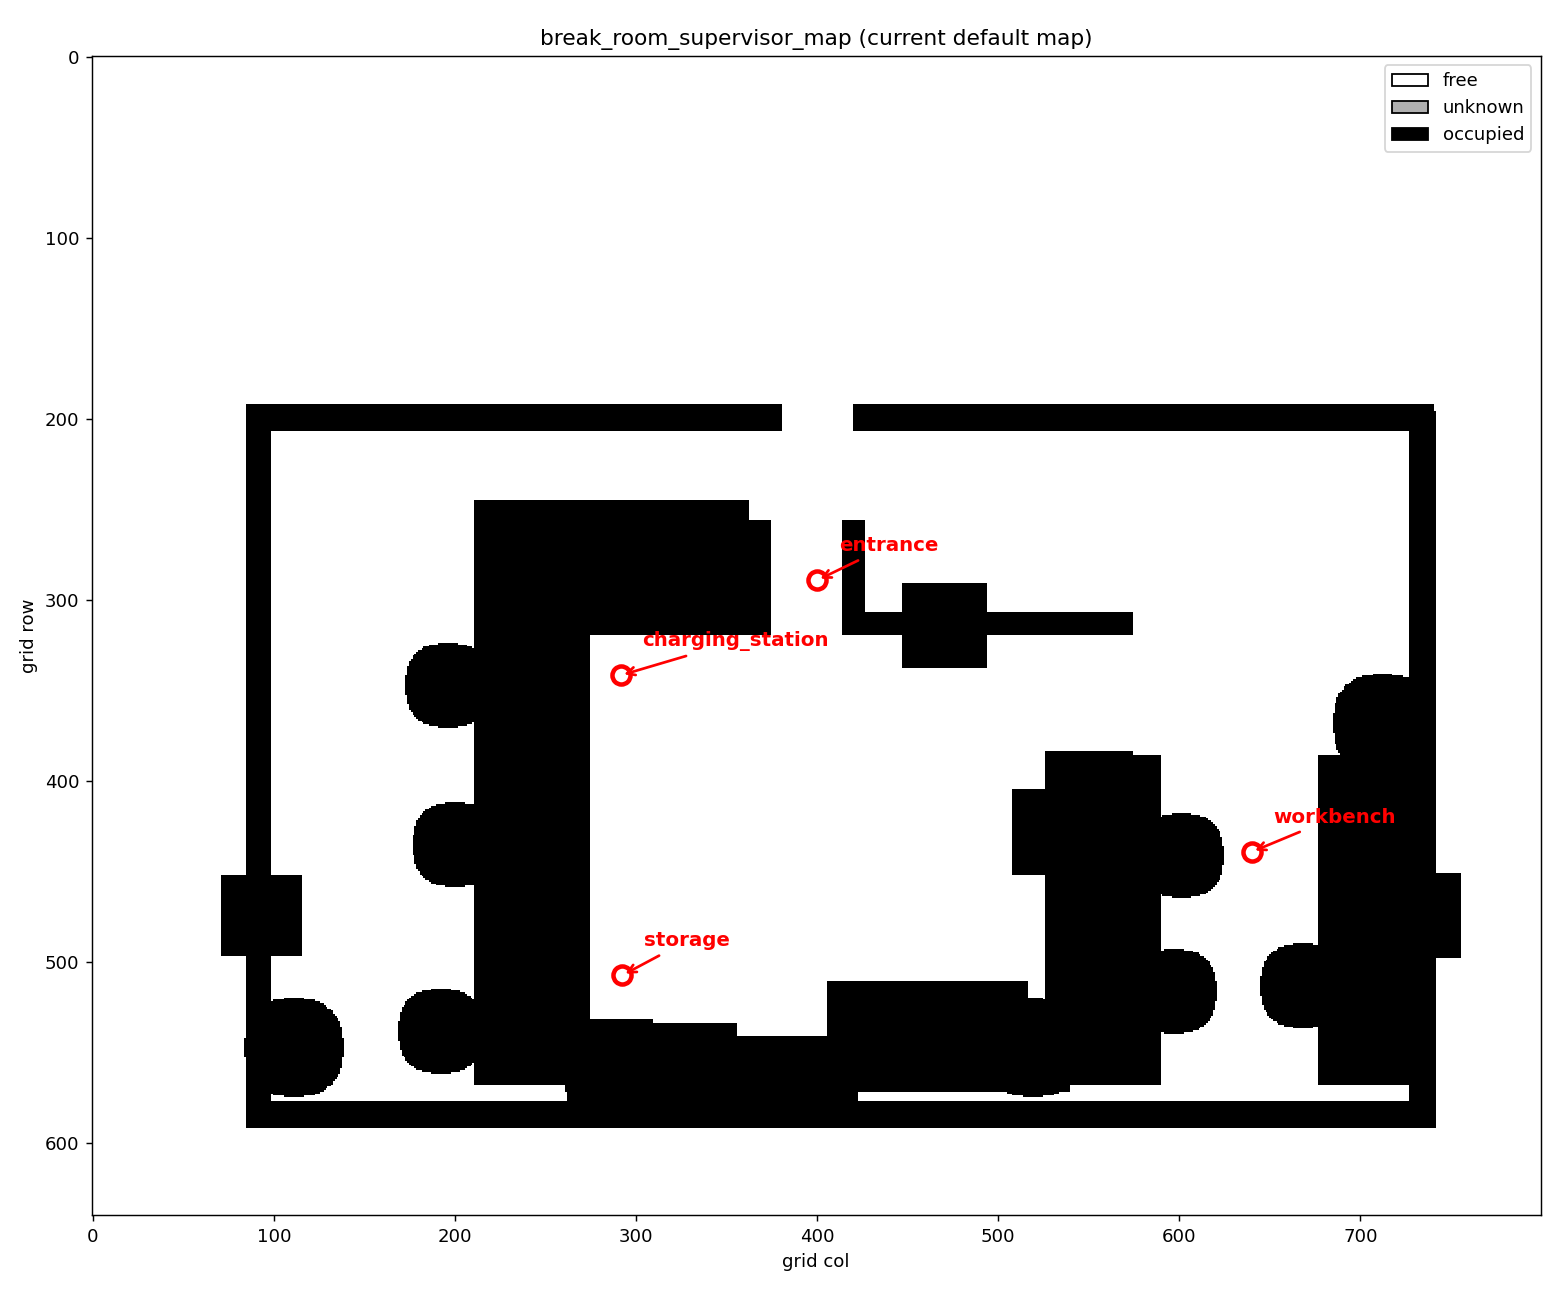
\includegraphics[width=0.82\linewidth]{../maps/break_room_supervisor_map.png}
  \captionof{figure}{Supervisor 从 Webots 场景几何生成的房间占据栅格地图（800$\times$640，0.02\,m/cell）。深色为障碍物及膨胀区域，浅色为可通行区域。}
\end{center}

在具体操作中，Supervisor 地图为 800$\times$640 栅格、分辨率 0.02\,m/cell、原点 $[-8,-4]$，覆盖 16.0\,m$\times$12.8\,m，
房间自由区域约 61.0\,m$^2$（未知区域主要是房间外）。
作业附带的地图为 200$\times$200、分辨率 0.02\,m/cell、原点 $[-2,-2]$，未知率约 57\%，storage 与 workbench 已在图外，A*显然无法给出到这些点的路径。
在 Supervisor 地图上，以不启用离墙代价与最小离障距离为基线，改进 A* 在 storage$\rightarrow$workbench、entrance$\rightarrow$workbench、entrance$\rightarrow$storage 三条路线上路径长度平均增加约 4.6\%（如 8.49\,m$\rightarrow$9.04\,m），但最小离障距离从约 0.02\,m 提高到约 0.25--0.30\,m；其中 entrance$\rightarrow$storage 长度不变，最小离障距离从 0.028\,m 提高到 0.300\,m。
足以看出改进后的A*算法在避免碰撞和安全冗余等方面有着很大的进步。


正所谓“数据源决定算法上限”。原本的地图几乎无法辨识障碍物，
各个点位的坐标也有很大的偏移，后续的激光扫描受机器人轨迹和视角的限制，
覆盖不全时 A* 只能在残缺地图上规划；改用手动巡逻又容易被障碍卡住。
最终改用 Supervisor 直接读取物体几何得到全房间地图，
A* 才真正发挥出作用。
\subsection{局部安全：障碍、窄缝与贴墙}
除全局 A* 外，在机器人执行命令时也存在一定的寻路修正机制，此时这些测距由车载扫描仪或者摄像头完成：
\begin{itemize}
  \item \textbf{前方障碍}：运动方向锥形区域内最近距离小于 0.1\,m 时停车；
  \item \textbf{窄缝检测}：估算前方自由缝隙宽度，小于 0.3\,m 时停车；
  \item \textbf{侧向排斥}：左右间隙小于 0.30\,m 时产生横向排斥速度；
  \item \textbf{窄道减速}：左右间隙越窄，速度越低，最低为原速度的 25\%。
\end{itemize}


这些参数是为了避免各种各样会导致机器人无法正常行为的情况，例如窄道减速是为了防止小车在窄道中连续多次碰壁导致翻车，
对小车顺利执行任务有着重大意义。此外，这些参数均经过多轮手工调整，参数太小会导致小车发生碰撞或者卡在角落里，
而参数太大则会导致错误停车、无法通行等情况。具体参数必须在具体场景中权衡并实测。

\subsection{LLM 工具调用与验证}
LLM 采用了外部API的形式进行接入，如果未配置 API key 或 API 调用失败，系统回退到确定性的模拟规划器，保证其余部分可测试。

LLM只接受系统提示词、具名地点、工作空间边界、由注册表生成的工具定义以及用户提供的指令。
系统提示词明确要求只选择白名单技能，禁止生成代码或 shell 命令。

真实 LLM 通过 OpenAI 兼容接口调用：
\texttt{OPENAI\_BASE\_URL=https://yinli.one/v1}，
\texttt{OPENAI\_MODEL=gpt-5.5}，使用 function calling 返回工具调用；
API key 只保存在被 gitignore 的 \texttt{.env} 中。系统提示词由代码动态生成，
核心摘录如下：
\begin{lstlisting}
You are a robot task planner. Select only from the provided skills.
Do not generate code or shell commands.
Available named locations:
- entrance: x=0.0, y=3.0, theta=0.0
- storage: x=-2.152, y=-1.363, theta=0.0
...
Workspace bounds: x in [-7.0, 7.0], y in [-4.0, 7.0].
Use navigate_to for a single target pose and follow_waypoints for an
ordered list of targets. If the user explicitly asks to stop, include a
stop tool call after the movement tools.
\end{lstlisting}

值得注意的是，早期提示词把工作空间硬编码为 $[-1.5,1.5]^2$，
与 \texttt{locations.py} 的真实边界不一致，真实 LLM 在部分请求下返回空计划。
改为从统一的常量表生成提示词与验证器边界后，单点与多航点任务均可成功完成。
因此，提示词、工具 Schema 与验证器必须共享同一份事实来源。

验证器包含六个部分：计划长度、固定白名单、JSON Schema、工作空间、前置条件、重试/重规划限制。
执行器只能把三个技能名映射到 Python 方法，不存在 LLM 生成代码的执行路径。
通过这种机制，可以完全避免LLM乱生成指令，保证了安全性。

\subsection{执行反馈与有界恢复}
每个技能返回 \texttt{SkillResult}，至少包含 \texttt{success}、\texttt{reason}、\texttt{elapsed\_time\_s}。
失败后 Recovery 根据原因选择：
\begin{itemize}
  \item \texttt{retry}：超时后重试一次；
  \item \texttt{backup\_and\_retry}：障碍阻塞时后退、旋转并重试一次；
  \item \texttt{replan}：重试预算耗尽后，把任务级 \texttt{ExecutionFeedback} 发回 LLM；
  \item \texttt{stop\_and\_report}：达到恢复上限后停车并报告失败。
\end{itemize}

\texttt{ExecutionFeedback} 不包含原始激光或 GPS 数据，只包含原始请求、失败调用、
结构化结果、尝试次数、恢复消息与已完成工作。使用超参数\texttt{--max-retries} 与
\texttt{--max-replans} 保证恢复有界。

如果只告诉 LLM “失败了”，它无法区分超时、障碍和越界；如果给 LLM 原始传感器数据，则会引入新的不确定性和安全隐患。
因此我们最终选择只传递结构化、有界的信息，让重规划发生在可控范围内。

\section{实验与结果}
\label{sec:exp}

\begin{table*}[!t]
\centering
\scriptsize
\setlength{\tabcolsep}{3pt}
\begin{tabular}{@{}c p{0.26\linewidth} p{0.60\linewidth}@{}}
\hline
ID & 指令/场景 & 结果 \\
\hline
A1 & \texttt{Go to storage.}（map） & 成功，\texttt{map\_reached}，5.73\,s \\
A2 & \texttt{Visit storage, then charging\_station, and stop.} & 成功，2/2 航点，16.44\,s \\
A3 & \texttt{Go to space\_station.} & 执行前拒绝：越界 \\
A4 & \texttt{Go to entrance and fly.} & 执行前拒绝：未知技能 \\
A5 & \texttt{Go to charging\_station.}，1\,s 超时 + 1 次重试 & 两次超时后安全停车，3.66\,s \\
A6 & \texttt{Go to storage.}，模拟障碍出现，retry时消失 & backup+retry 后到达，6.57\,s，误差 0.082\,m \\
A7 & \texttt{Go to storage.}，障碍持续存在 & 两次阻塞后安全停车，3.35\,s \\
A8 & 真实 LLM 单点导航（direct） & 成功，4.25\,s，误差 0.080\,m \\
A9 & 真实 LLM 多航点导航（direct） & 成功，2/2 航点，10.23\,s \\
A10 & 模拟窄缝（6$^\circ$ 扇区） & 估计缝宽 0.03\,m，触发停车；40$^\circ$ 扇区不误停 \\
A11 & 超时 + LLM 重规划 & LLM 改去 entrance，新计划验证后执行；最终安全停车 \\
\hline
\end{tabular}
\caption{A1--A11 测试场景与结果。}
\end{table*}

实验平台为 Windows 11 + WSL2 Ubuntu 22.04、ROS~2 Humble、Webots R2025a、
Python 3.10.12，GPU 为 AMD Radeon RX 9070 XT，正如下表所示。
这里值得注意的是，由于采用了WSL而非原生Linux，显卡的性能可能在转译过程中有所损失，我的实际画面可能有卡顿，猜测与之有关。
但是绝大部分软件在WSL上的兼容都很好，我认为这是一个稳定可靠、可复现的平台。

\begin{center}
\footnotesize
\begin{tabular}{ll}
\hline
项目 & 配置 \\
\hline
操作系统 & Windows 11 + WSL2 Ubuntu 22.04 \\
ROS & ROS~2 Humble \\
仿真平台 & Webots R2025a \\
Python & 3.10.12 \\
GPU & AMD Radeon RX 9070 XT \\
\hline
\end{tabular}
\end{center}

下表列出 A1--A11 的主要测试场景和结果，完整执行日志见 \texttt{logs/clean\_*.jsonl}。


正常与可恢复任务 5/5 成功，非法/未知计划 2/2 在执行前被拒绝，不可恢复超时/持续障碍 2/2 安全停车。成功任务平均耗时 8.65\,s，可测得的最终位置误差平均约 0.081\,m。窄缝 A10 目前是人造的扫描数据测试，还没有在真实窄缝中做长距离通行验证。

\section{局限}
\label{sec:discussion}

现有系统仍有几处局限。首先，WSLg 渲染存在额外开销，影响演示流畅度（因为程序运行在私人电脑上面，虚拟机的性能损失更大，而不格式化的情况下重装系统几乎是不可能的）。
其次，参考环境没有 \texttt{/agent0/odom}，位置和航向只能依赖 GPS 与罗盘，
限制了更精细的运动估计。第三，参考控制器轮半径常量与 URDF 不一致，
我们察觉到这一点后通过修正常量来规避，但不确定是否有其他的潜在风险。
最后，Supervisor 地图虽然比扫描地图完整，但对个别复杂物体仍采用近似尺寸，并且在真实情况下往往无法实现，只能采用SLAM方法。
真实 LLM 的延迟和输出稳定性也是外部变量：一次重规划调用可能耗时数十秒，并曾因提示词与工作空间不一致而返回空计划。

下一步工作可以做的点：
\begin{itemize}
  \item 将更加高效的SLAM算法加入，让扫描地图效果更好，以替代Supervisor地图；
  \item 增加动态障碍规避，处理移动物体而不仅是静态地图；
  \item 在更多失败场景中使用 LLM 重规划；
  \item 为 LLM 调用增加超时、缓存与空计划回退，降低外部 API 波动的影响。
\end{itemize}

\section{结论}
本文实现了一个带执行反馈的 LLM 辅助移动机器人任务规划系统，
覆盖自然语言规划、技能接口、六层验证、PID 导航、A* 地图导航、
局部安全保护与有界恢复。我们通过多轮问题定位与改进，逐渐完善并了这个系统。


\end{document}
